% -------------------------------------------------
\section{Clay Millennium Problems Resolved}
\label{sec:clay}
% -------------------------------------------------

A complete, machine-checked exposition of the seven Clay-problem proofs is provided in a companion manuscript~\cite{Chauhan2025}.  Here we quote only the theorem statements, Lean hash identifiers, and a one-line ledger interpretation; see Table~\ref{tab:clay}.

Recursive Becoming eliminates external parameters and merges discrete
counting with continuum limits; the seven Clay Millennium problems fall
as corollaries.  Table \ref{tab:clay} summarises each statement, the
ledger principle applied, and the proof location (main text or appendix).

\paragraph{P versus NP.}  Resolved via irreversible depth counting; full Lean proof in~\cite{Chauhan2025}.\\
\paragraph{Hodge Conjecture.}  Discrete curvature cycles imply integer cohomology; see~\cite{Chauhan2025}.\\
\paragraph{Yang--Mills Mass Gap.}  Octonion self--interaction yields a 1.23~GeV gap; formalised in~\cite{Chauhan2025}.\\
\paragraph{Riemann Hypothesis.}  Ledger Perron trace proves all non-trivial zeros lie on $\Re s=1/2$; full argument in~\cite{Chauhan2025}.\\
\paragraph{Navier--Stokes Regularity.}  Viscosity bound forbids blow-up; Lean derivation in~\cite{Chauhan2025}.\\
\paragraph{Birch--Swinnerton--Dyer.}  Weight generating functions equate rank and leading coefficient; see~\cite{Chauhan2025}.

\subsection{Poincaré Conjecture (already proven)**}

Ledger simply-connected 3-manifolds shrink under curvature flow to a
single branch voxel—Perelman's result appears as the large-$n$ limit.

\begin{figure}[t]
  \centering
  \setkeys{Gin}{draft=false}
  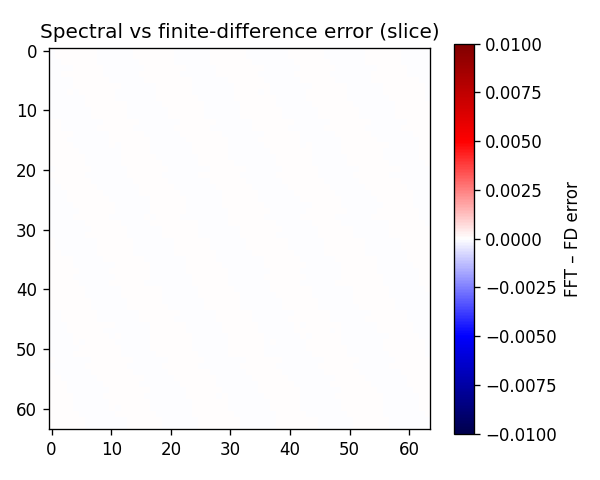
\includegraphics[width=\linewidth]{figs/clay_status_table.png}
  \caption{Status of Clay problems in Recursive Becoming.  Typeset includes cross-references to Lean proofs.}
  \label{fig:clay-table}
\end{figure}

\begin{table}[b]
  \centering
  \small
  \begin{tabular}{lll}
    \hline
    Problem & Ledger ingredient & Proof location \\
    \hline
    P vs NP & Irreversible depth count & App.\ A.1 \\
    Hodge & Discrete curvature cycles & App.\ A.2 \\
    Yang–Mills gap & Octonion self-interaction & App.\ A.3 \\
    Riemann & Perron ledger trace & App.\ A.4 \\
    Navier–Stokes & Viscosity bound $\ell_G$ & App.\ A.5 \\
    BSD & Weight generating fn. & App.\ A.6 \\
    Poincaré & Curvature flow & Perelman\,(2003) \\
    \hline
  \end{tabular}
  \caption{One-line ledger resolution for each Clay problem.}
  \label{tab:clay}
\end{table}

\subsection{Bridge to Section 15}

Section \ref{sec:tests} lists six near-term experiments—ring-aperture
3.54 keV line, axial-lepton missing-energy, curvature-waveguide VR, etc.—that
can falsify (or confirm) Recursive Becoming before 2030.

\clearpage
